\begin{document}

\def\title{Linearization}

\newcommand{\qitem}{\qpart\item}

\renewcommand{\labelenumi}{(\alph{enumi})} % change default enum format to (a)
\renewcommand{\theenumi}{(\alph{enumi})} % fix reference format accordingly.
\renewcommand{\labelenumii}{\roman{enumii}.} % second level labels.
\renewcommand{\theenumii}{\roman{enumii}.}

\maketitle

\vspace{0.5em}


\begin{qunlist}

% {\Large \textbf{Mechanical:}}
\qns{Linear Functions}
\qcontributor{Sirej Dua}


\begin{enumerate}

\qitem  If $f$ is a linear function, is it true that $f(ax) = af(x)$?

\sol{
	Yes.
}




\qitem  If $f$ is a linear function, is it true that $f(x + y) = f(x) + f(y)$?

\sol{
	True.
}



\qitem If $f$ is a linear function, is it true that $f(ax + \frac{1}{b}y) = af(x) + \frac{1}{b}f(y)$?

\sol{
	True.
}

\qitem Is the following function linear? $f(x) = ax,\ a \in \R$
\sol{
	Yes. 
}


\qitem Is the following function linear? $f(x) = x^2$

\sol{
	False.

}

\qitem  Is the following function linear? $f(x) = ax+b,\ a,b \in \R$

\sol{
	False. But the function is affine.
}









\end{enumerate}
% {\Large \textbf{Mechanical:}}
\qns{Linearizing a Function}
\qcontributor{Sirej Dua}


\begin{enumerate}

\qitem   Let $f(x) = x^2 + 3$. Linearize $f(x)$ about the DC operating point $x^* = 0$, as $f_L = mx + b$. What are $m, b$?

\sol{
	$m = 0$. This is because $m = \left. \frac{d}{dx} f(x) \right|_{x^*=0} = \left. 2x \right|_{x^*=0} = 0$.

	$b = 3$, since $f(x^*) = 3$.
}


\qitem  Take $f_L$ that you computed in the previous part. What is $f_L(1)$?

\sol{
	$f_L(1)= 3$.
}



\qitem What is $f(1)$?

\sol{
	 $f(1)= 4$.
}

\qitem What is the relative error, $\frac{f(1) - f_L(1)}{1}$?
\sol{
	    $\text{relative error} =  $
	$\frac{f(1) - f_L(1)}{1} = 1$. 
}


\qitem What is $f_L(0.5)$?

\sol{
	$f_L(0.5)= 3$.

}

\qitem What is $f(0.5)$?

\sol{
	$f(0.5)= 3.25$.
}

\qitem What is the relative error, $\frac{f(0.5) - f_L(0.5)}{0.5}$?

\sol{
	$\frac{f(0.5) - f_L(0.5)}{0.5} = 0.5$.
}




\qitem What is $f_L(0.25)$?

\sol{
	$f_L(0.25)= 3$.

}

\qitem What is $f(0.25)$?

\sol{
	$f(0.25)= 3.0625$.

}

\qitem What is the relative error, $\frac{f(0.25) - f_L(0.25)}{0.25}$?

\sol{
	$\frac{f(0.25) - f_L(0.25)}{0.25} = 0.25$.
}


\qitem What is the relative error for $f_L$? Specifically, what is $\frac{f(x) - f_L(x)}{x}$ symbolically?

\sol{
	The relative error is $x$.
}


\end{enumerate}
\qns{Graph Linearization}
\qcontributor{Sirej Dua}
 
 I linearized a function, and printed a graph of what the linearization, but then I carelessly I lost the original function. This is a plot of the linearization.

    Which of the following functions, linearized about $x=0$, could have been my function? \\

    1. $3x + \cos x - 1$, \\
	2. $3x$,\\
	3. $x + 2e^x - 2$,\\

    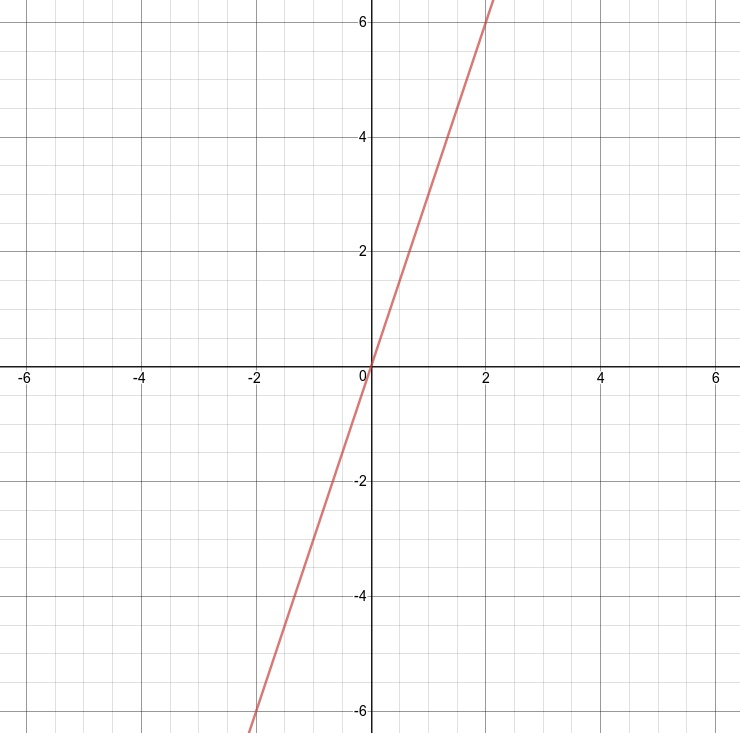
\includegraphics[scale=0.4]{\bank/linearization/figures/line.png}

    
	\sol{
	All three can be linerized about $x=0$ to the function in the graph.



	% TODO: detailed explanation
	}


\end{qunlist}

\end{document}
